\documentclass{article} % For LaTeX2e
\usepackage{hyperref}
\usepackage{url}
\usepackage{times}
\usepackage{bbm}
\usepackage{amsmath, amssymb,, epsfig}
\usepackage{sectsty}
\usepackage{pdfpages}
\usepackage{indentfirst}
\usepackage{graphicx}
\usepackage[margin=1in]{geometry}
\usepackage{times}
\usepackage{bbm}
\usepackage{amsmath, amssymb,, epsfig}
\newcommand*{\QEDA}{\hfill\ensuremath{\blacksquare}}
\usepackage{sectsty}
\usepackage{pdfpages}
\usepackage{indentfirst}
\usepackage{graphicx}
\usepackage[margin=1in]{geometry}

\title{NBA Predictions}

\author{Lee Richardson (lrichard) Daren Wang (darenw) \\ Chi Zhang (chiz2) Xiaofeng Yu (xiaofen1)}  

\newcommand{\fix}{\marginpar{FIX}}
\newcommand{\new}{\marginpar{NEW}}

\begin{document}

\maketitle

\begin{abstract}
Last year, the defending champion Miami Heat lost consecutive games against the lowly Detroit Pistons and Milwaukee Bucks. While this two game stretch was certainly unlikely, it exemplifies the inherent randomness present in NBA basketball games. In this paper, we examine how well we can predict the outcomes of individual games using various machine learning algorithms. Specifically, we see that we can accurately predict around 70\% of individual games, and that simple, interpretable classifiers such as Logistic Regression and Naive Bayes work the best. We then use these predictions to simulate full NBA seasons, which land us in the top 15 of all publicly available NBA projection systems \cite{projections}. Finally, we see that the recently developed Regularized Adjusted Plus Minus (RAPM) statistic is a better predictor than the more commonly used box score statistics. 
\end{abstract}

\section{Introduction}
	In recent years, there has been lots of talk in NBA circles regarding the rise of statistical analysis\cite{revolution}. This has been in the works for years, starting with Dean Oliver's Basketball on Paper \cite{bop}, which was for a long time the cornerstone of basketball statistics. Recently, new data has become publicly available, most notably play by play data which provides a record of each event, when they happened, and which were on the floor when they happened. This is in contrast to the more commonly known Box Score statistics, which are useful, but have less information than play by play data. In fact, every box score statistic can be inferred from play by play data. Within the last few seasons, camera's were installed in every NBA arena \cite{sportsvu}, which track the location of the ball and each player 10 times per second. However, this camera data is proprietary, and it will be awhile before it's released and people are able to make sense of it. \\

	In this paper, we harness all publicly available data sources to predict the outcomes of NBA basketball games. In section two, we will look at previous attempts at the problem and provide a more detailed description of RAPM. Next, we will describe how we compiled our database, and give information on how one could access it. In section four, we describe our efforts in predicting games using various algorithms, features, and model selection techniques. Then we discuss how we used our game predictions to simulate full seasons, and compare our results with other projection systems. We conclude with a discussion of what we learned and ways we can improve our predictions. 

\section{Related Works}
	%%% TALK ABOUT NBA ORACLE AND DATA MINING TO COMPARE PREDICTION ACCURACIES
	We looked into the literature to see if anyone had worked on the same or similar problems. From this, we found a few papers, specifically \cite{nba_oracle} and \cite{data_mining}, which also attempted to predict the outcomes of NBA games. These papers used linear and logistic regression, naive Bayes, neural networks, and Support Vector Machine's as their classifiers, and used mainly box score statistics as features. They also used the same loss function (zero one loss) that we are proposing, which gave us a target test error to shoot for when implementing our algorithms. Specifically, \cite{nba_oracle} achieved the highest single season classification rate of 73\% in the 1996 season using linear regression. All of the other season/algorithms combinations had error rates from the mid 60's to low 70's. \\

	%%% DELVE INTO THE RAPM PAPER TO EXPLAIN WHY IT'S SO GOOD
	One advantage we believe we have compared with these groups is that we have a more robust feature set, most notably, we have RAPM. RAPM has been anointed by many as the next big thing \cite{bigrpm} in the basketball statistics community, and we hope that using it as a feature will help differentiate our attempts at game classification. Taylor et al. have a great explanation of the statistic \cite{rpm}, but the basic idea is to split each game into miniature games, each one occurring in time periods when there's no substitutions. The final dataset consists of the score margin of each miniature game, and indicator variables for each player involved (+1 for offense, -1 for defense). Then a regression is ran (people are now using ridge regression, which is why the R in RAPM stands for Regularization), and the coefficients represent each players individual contribution per 100 possessions on offense and defense. RAPM adjusts for flaws in original plus minus, by correcting for the fact that player totals are heavily influenced by the play of his opponents and teammates, and by pooling information from previous seasons to reduce the margin of error. 

\section{Dataset}

\subsection{Challenges for dataset preparation}
We encountered several challenges in the dataset preparation phase.

\begin{itemize}
\item There are currently no ready-made data sources for our experiments. What we can find is several websites on NBA games. Since we are interested in statistics of thousands of games with hundreds of players, it's not realistic to acquire those data manually from websites.
\item Data sources from different websites have to be merged using a uniformed format. Different websites may treat player names and season labels differently. For example Roger Mason Jr. and Roger Mason are in fact same person from different websites, while uta and utah are different abbreviations for the Utah Jazz.
\item Data needs to be stored in a proper manner so that our future experiments can be implemented based on a uniformed and easily accessible API.
\end{itemize}

To meet those challenges, we are writing our own web crawlers to get data from websites, then made lots efforts on ETL on ensure different data sources were properly combined. Finally we stored all data into a SQLite database.
It's worth mentioning that we are making our dataset public online at \\
\url{https://github.com/leerichardson/game_simulation/blob/master/nba_rRegression_chi/nba.db}\\
Hopefully this will save some effort for anyone interested in research on NBA statistics in the coming years. \\

\begin{figure}
		\centering
		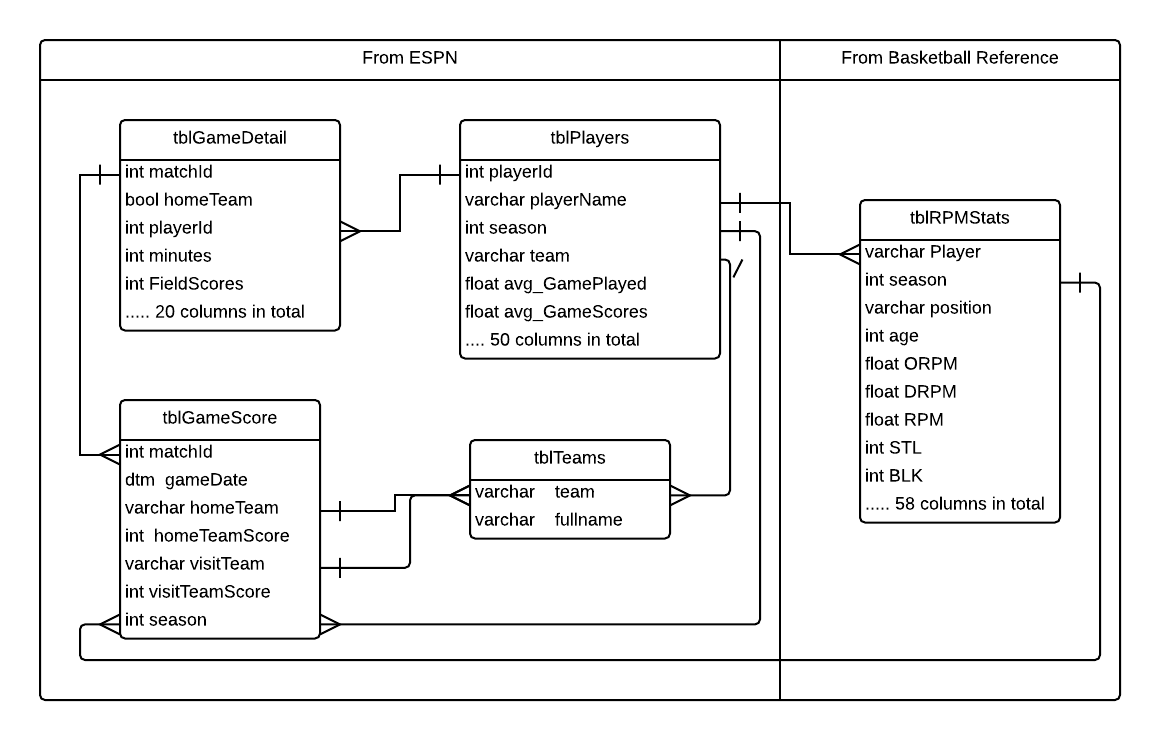
\includegraphics[width=150mm, height=120mm]{sqliteERDiagram.png}	
		\caption{Entity - Relationship graph for SQLite database. The database follows the third normal form to ensure there is no redundancy. Two main data sources of the dataset are ESPN and Basketball References websites. Lines between tables indicate the primary key - foreign key relationship between dataset entities.}
		\label{fig:database}
\end{figure}

\subsection{Data Sources}
	We did not have a processed dataset for this project, so we created our own database. The three main sources we used were ESPN's NBA website \cite{espn}, basketball reference \cite{bball_ref}, and a new website from Jeremias Engleman \cite{rpm_data}. We used the ESPN data to get information about all NBA games from 2009-2014. This includes the game score, the home and away teams, the players involved and their individual statistics. Also from ESPN, we have a player database, which has 50 individual statistics for each player in each season. There are 7139 games in this dataset. \\

	The next data source we used was basketball reference \cite{bball_ref}. The main reason we used this site is because they have a larger individual player database, with information dating back to the 1950's and more advanced statistics, such as the widely used Player Efficiency Rating (PER), compared with just box score statistics provided by ESPN. \\

	The final source we used was from a website put together by Jeremias Engleman \cite{rpm_data}. This site has RAPM statistics described above, dating back to the 1980's. This statistic has been widely adopted in the NBA statistics community, and it's one of the few trustworthy stats which provides an individual assessment of defense. As we see below, RAPM is a very useful feature in predicting game outcomes. \\

	%%% WEB CRAWLERS
\subsection{Web Crawlers}
	To obtain all of these datasets, we used web-crawlers to pull them off their websites. All of these scripts can be found in our Github repository \cite{gitrepo}. For the ESPN data, we used the BeautifulSoup package in the Python language. For the other two datasets, we used the XML package in R. \\

	%%% TALK ABOUT MERGING SOURCES 
	\subsection{Merging Sources into One Database}
	One of the major obstacles in our project has been combining these three data sources into one single database. The ESPN dataset had both match and playerID's for each game, so merging the game statistics with the ESPN player database wasn't very difficult. However, the basketball reference and RAPM dataset didn't have these identifiers, so it was more challenging to put them together. We ended up using the player's name, team, and season to join both of these datasets together with ESPN. Some common problems we had were inconsistent spelling of names in different datasets, inconsistent team names, teams have changed cities, etc.. In the end, we were able to sync most of the idiosyncrasies between the three datasets, which is important because it gives more interesting features than just box score statistics. That being said, we don't doubt that there's still be further cleaning to be done, as it's hard to catch all of the idiosyncrasies in these three separate datasets. \\

\section{Experiments}
	%%% TWOFEATURE MATRICES/.. LARGE AND JUST RAPM/PER
	\subsection{Training and test datasets}
	We devoted a substantial amount of time to construct features that can be used to train the model. The features are constructed using of both the RAPM dataset and the ESPN data (recall that the ESPN data provide basic statistics such as the average number of points per game or the average number of rebounds per game for a given season). To create the features, we considered each match and listed the players on each team, then we merged the players' statistics from the previous season with the results in the matches of the current season. We then add up  the players' statistics to form statistics for home teams and away teams. In the computation of the offensive and defensive RAPM statistics of each team, the players' average minutes per game from the previous season were used as weights. To illustrate, suppose that there are $n$ players in each team, with the $i$-th player  playing $m_i$ minutes per game and having RAPM score $r_i$ in the previous season. Then, the weight for the $i$-th player and the team offensive RAPM are determined as:

	\begin{align*}
		w_i &= \frac{m_i}{\frac{1}{n}\sum_{i=1}^{n} m_i} \\
		\text{Team Offensive RAPM} &= \frac{1}{n}\sum_{i=1}^{n} w_i \times r_i.
	\end{align*}

	%%% TABLE OF EXAMPLE MATRIX %%%
	\begin{table}[ht]
	\centering
	\begin{tabular}{rrrrrr}
	  \hline
		ORPM\_home & DRPM\_home & ORPM\_away & DRPM\_away & homeWin \\ 
	  \hline
		-0.28 & 0.89 & 0.65 & 0.18 & 1 \\ 
	  	-0.28 & 0.89 & 1.15 & 1.05 & 1 \\ 
	  	-0.29 & 0.99 & -1.44 & 0.12 & 1 \\ 
	  	 0.03 & -0.66 & 0.04 & 1.09 & 1 \\ 
	  	 0.28 & 1.26 & -0.81 & -0.20 & 0 \\ 
	  	-0.75 & -0.46 & 0.51 & 1.02 & 1 \\ 
	   \hline
	\end{tabular}
	\caption{A look at what our training and test datasets look like. The first four columns are features and the 5th column (indicating whether or not the home team won the game) is our label.}
	\label{table:matrix}
	\end{table}
Before training the model, we tried to understand how the features that we constructed related to the game results.
In Figure \ref{feats}, the left plot has the home team RAPM on the $x$ axis and the away team RAPM on the $y$ axis. The plot suggests that the game results are not linearly separable using RAPM. However, the green dots (corresponding to the losses for the home team) are close to a Gaussian distribution centered above the diagonal line of the plot, while the red dots are centered below the diagonal line. If one takes the diagonal line as the decision boundary, the majority of the data points are correctly classified. The right plot displays the teams' RAPM in wins compared with the teams' RAPM in losses. The horizontal line at the middle of each box corresponds to the sample mean. The top and bottom ends of the boxes are the empirical first and third quartiles, respectively. From the plot, one observes that RAPM is higher in wins than losses, suggesting that RAPM is a relevant feature.


\begin{figure}[h]
	\centerline{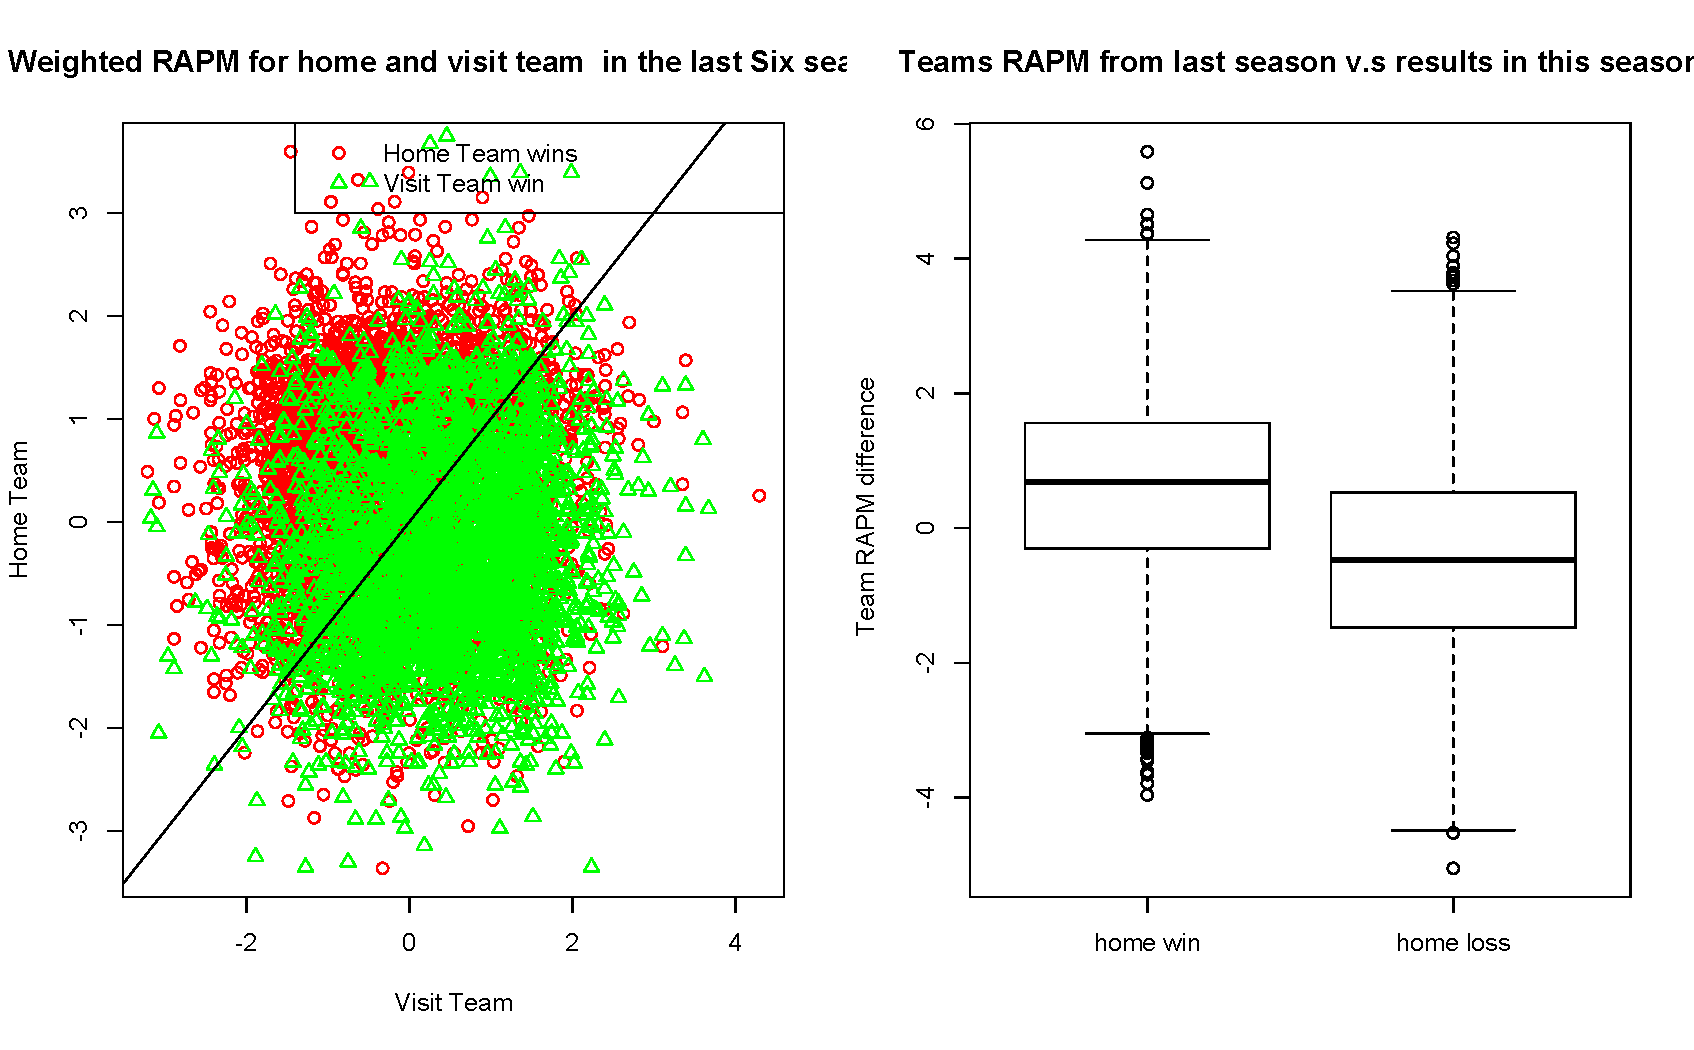
\epsfig{file=features.pdf, width=7in,height=3.25in}}
	\caption{Left: visit team RAPM against home team RAPM; the green dots indicate visit team wins while the red dots indicate home team wins. Right: box plot of RAPM; the $y$ axis represents the difference in RAPM between the home team and the visit team.}
	\label{feats}
	\end{figure} 
	
	
	\subsection{Algorithms and feature selection}
	 We tried different models based on the features that we constructed to predict the game results. For each model, we split our dataset into a training set and a test set. 
	 We trained our model using available data from the previous season and we used the model to predict the game results of the particular years in which we are interested. For example, to predict the game results for the 2010 season, we trained the model using data from seasons 2008 and 2009. %Chi's plot pleas
	
	\begin{figure}[h]
	\centerline{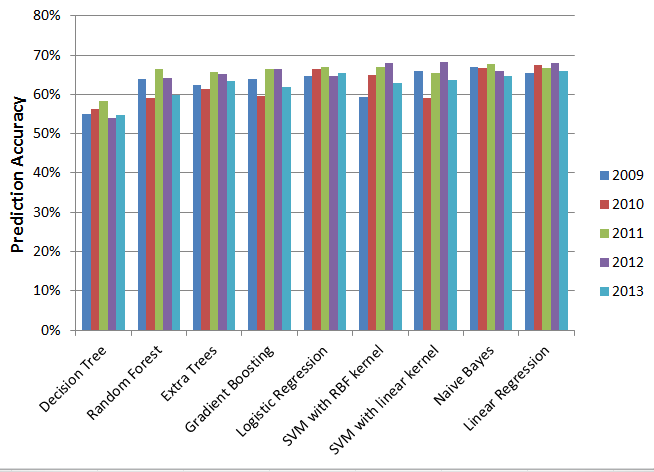
\epsfig{file=linear2.PNG, width=6in,height=4in}}
	\caption{Test accuracy of each algorithm }
	\label{diffmodel}
	\end{figure} 
	
	
	\subsection{A discussion of the algorithms}
	To predict the game results, we used algorithms such as linear regression, logistic regression, naive Bayes, SVM, and decision trees.
	\begin{enumerate}
	\item \textbf{Linear Regression.}
          In order to fit the linear regression model, the game results are denoted as 0 and 1 (with 1's denoting home team wins). The fitted model is described in terms of a vector  of estimated coefficients (one for each feature) which we denote $\hat \beta$. To predict new games results using this model, one evaluates $\hat \beta^{T} X_{\text{test}}$, where $X_{\text{test}}$ corresponds to the vector of features for the new games. We predict that the home team wins if $\hat \beta^{T} X_{\text{test}} \ge 0.5$, and that the home team loses otherwise.
	\item \textbf{Logistic regression.} Logistic regression is particularly useful when the outcome is binary. As before, we use 0 and 1 to denote wins and losses, and we predict that the home team wins a new game if the predicted value for that game is greater than or equal to $0.5$. Predicted values from a logistic regression are estimates of the probability that the home team wins. Thus, predictions from the logistic regression model are easily interpretable.
	\item \textbf{Naive Bayes.} The naive Bayes classifier is a simple probabilistic classifier that selects the hypothesis that maximizes a posterior probability. The underlining assumption for naive Bayes classifier is that all the features are independent. Although in our case the features are not independent, the naive Bayes classifier performs relatively well compared with the other models. 
	\item \textbf{SVM.}  A Support Vector Machine is a non-probabilistic classifier. We tried different kernels, and Figure \ref{diffmodel} displays the highest model accuracy achieved by the SVM among the kernels that we considered. Note that even though different kernels generate different decision boundaries, none allows to exactly classify all of the data points. For this reason, we use soft margin to train the model.
	\item \textbf{Decision tree.} A decision tree is useful when one needs a good way to split a dataset with many features. In our case, there are 44 features overall. In order to avoid overfitting, we choose the subtree that minimized the regularized training error, defined as the sum of the training error and $\lambda |T|$. Here, $|T|$ denotes the size	of the tree while $\lambda$ is a penalty parameter which is selected using cross-validation.
	\end{enumerate}

		Figure \ref{diffmodel} displays the test error of different algorithm. The linear model appears to have the best accuracy.  Note that, on the basis of the discussion above, the linear decision boundary were expected to perform well. The test accuracy plot confirms with this conclusion.\\
	

	
	
	
	
	\subsection{Feature selection}
	In this section we discuss feature selection. There are 44 features for each model. Feature selection can  prevent overfitting and thus improve prediction accuracy. We discuss feature selection for the linear regression model. For the  linear regression model, we perform feature selection by using lasso regularization and a stepwise AIC procedure. In the lasso regression, the effective degrees of freedom $\lambda$ are chosen to minimize the generalized cross validation error.  In the stepwise AIC procedure, we set the minimum model to be the model including only the intercept term and the maximum model to be the model including all of the 44 features. At each step of the stepwise AIC procedure, a feature is included or dropped from the current model in such a way to give the highest decrease in the AIC score until no further changes in the AIC score occur.  
			\\
			\begin{table}[ht]
	\centering
	\begin{tabular}{rrrrrr}
	  \hline
		 & Full model (linear) & & Lasso & & AIC \\ 
	  \hline
		2009 & 0.6544715 && 0.6658537 && 0.6617886  \\ 
	  	2010 &0.6739837  &&0.6853659 &&0.6788618    \\ 
	  	2011 & 0.6676768 & &  0.6626263 &&  0.6717172  \\ 
	  	2012 &0.6786005& & 0.6712775 && 0.6818552  \\ 
	  	2013 & 0.6601626 && 0.6634146 && 0.6601626  \\ 

	   \hline
	\end{tabular}
	\caption{A look at how feature selection improves the prediction accuracy.}
	\label{table:matrix}
	\label{featsel}
	\end{table}
	\\
	According to Table \ref{featsel}, stepwise AIC found a model with higher accuracy. The absolute difference in accuracy between the original model model and the selected model are not significant. However, the best prediction accuracy known is up to 70$\%$, while if one always predicts home team win, the accuracy is around 60$\%$. The improvement is not negligible.
\\ \\	We also note that both the lasso and the stepwise AIC procedure identify the overall team weighted RAPM as the most important predictive feature. This is confirmed by the fact that the stepwise AIC procedure starting with the null model selects home and away RAPM as the first two features that should be included in the model. Moreover, the coefficient of the  Weighted RAPM didn't shrink to 0 after the lasso and this is another indication that these feature is more relevant than the others.	
\section{Simulation}	

\begin{figure}
  \centering
  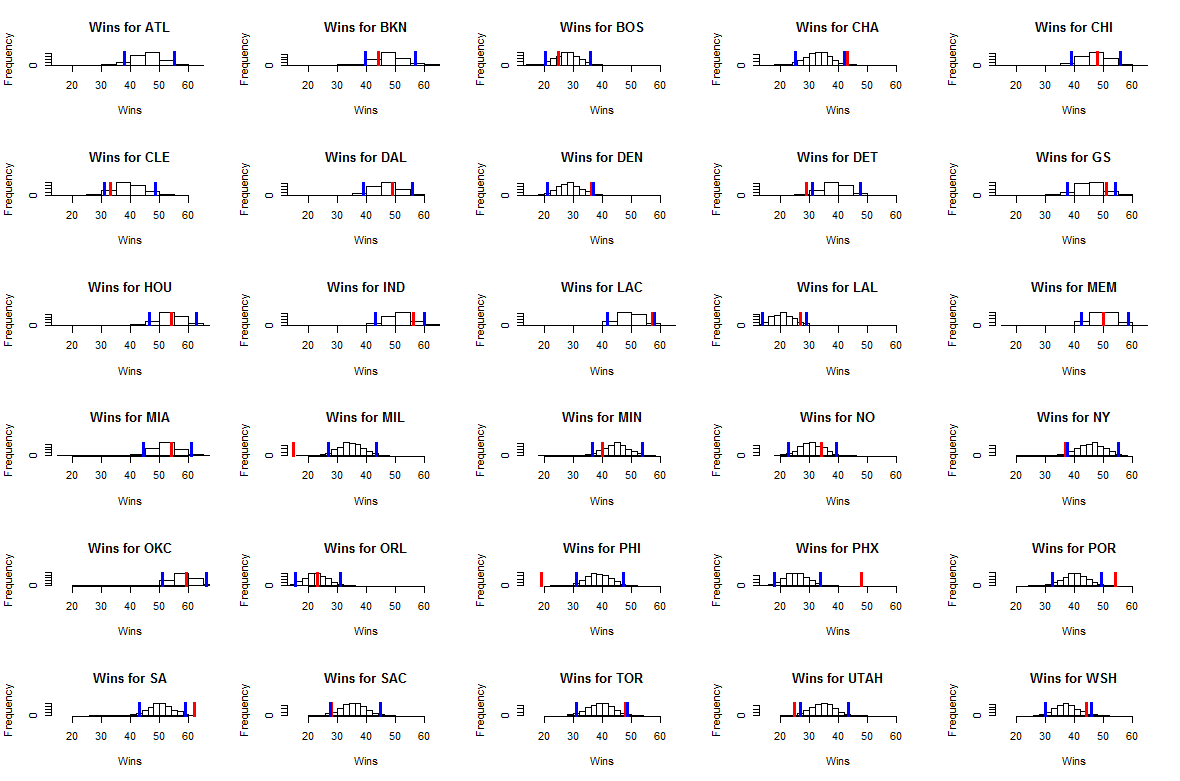
\includegraphics[height=15cm, width=15cm]{season_wins.png}
  \caption{Distribution of wins for each team from simulating the 2013 NBA season 1000 times, using probabilities from our best Logistic regression model. The blue lines represent our confidence intervals whereas the Red lines represent the actual number of wins for each team. Our simulations trapped the true number of wins in 70 \% of our intervals.}
  \label{fig:simulations}
\end{figure}

In order for the various classifier's to predict which team would win each game, they generate probabilities for each team (class), and predict the maximum. Another natural way to utilize these probabilities is to use them to simulation the entire season. Specifically, by generating Uniform(0,1) random variables, we were able to stochastically determine the outcome of each game, and simulation each game in a season. Then we simulated the season 1000 times to obtain the distribution of predicted win totals for each team. Figure \ref{fig:simulations} shows the win distributions for each team, using logistic regression for the 2013-14 season. Out of the two best classifiers (Naive Bayes and Logistic Regression), logistic regression performed much better in these simulations, using both the Root Mean Squared Error (RMSE) and Median Absolute Deviation (MAE) loss functions. This is because the game probabilities generated by Naive Bayes were much more extreme than logistic regression. While this doesn't effect classification as much since we're only selection the maximum, the exact probabilities matter in a more complicated function such as the result of simulating a complete season. To see how sensitive the simulated seasons are to these probabilities, consider the standard deviations of the number of predicted wins for each team using Naive Bayes and Logistic Regression. For Naive Bayes, they were 16.12 and 17.07, compared with 9.66 and 9.68 for logistic regression. This shows that the win totals predicted by Naive Bayes were much more extreme than logistic regression. \\

Forecasting how many wins each time will get during a seasons turns out to be a much more popular task than computing test errors, so we were able to compare our projections to lots of other systems using our RMSE loss function (which is commonly used by in the basketball analytics community \cite{projections}). Our RMSE for 2012 was 7.54 and 9.7278 in 2013. This would be in the top 20 for the past two seasons. Had we used Naive Bayes as opposed to Logistic regression, our system would have consistently performed in the bottom five. 


\section {Conclusion}
%% General Theory for How to clasify. Why is predicting the outcomes of seasons harder?
In the end, it seems that sticking with a simple classification algorithm yields the best accuracy in forecasting NBA games. It's clear that the two factors have the largest impact on each game are home court advantage and the quality of each team. Imagine that there's some perfect measure of the quality of each team, and that two teams are identical. In this situation, you should always pick the home team to win. The question then becomes, how much better does the away team have to be than the home team in order to choose them to win? Figuring out where to draw this line seems like the way to get the best performance out of classification algorithms. Obviously, since there's no way to know the exact quality of each team, this will be an estimate and is not an exact science. \\

%% Discuss why other systems bear us. (Projections, more developed, more nuances built in, etc...) Hollinger won, had been doing it the longers, mainly with PER
In terms of simulating seasons, it seems that more conservative estimates, such as those yielded by logistic regression, work better than more extreme predictions. For this endeavor, there were more public predictions available to compare our results with, and we see that while our system performs well, it did not approach some of the best publicly available systems. For instance, John Hollinger, who was recently hired by the Memphis Grizzlies, had the best projection system in 2012. He has been doing this for around 5 years, and written various books on the subject, so it makes sense his system would have better performance than ours, just based on experience. As we discuss below, there's many nuances that could be built into a projection system to make it more accurate, and since we only spent a semester on this project, there wasn't enough time to incorporate everything we hoped to include. \\


%% Why was 2013 so much less predictable than other years. Especially since we had the MOST training data. This gives some evidence to the theory that randomness may impact the results of these games more than a fancy classifier. sometimes the underdog will just win more. 
One interesting finding that came out of our report was how much lower our test error was in the final season, 2013. This is counter to what one would expect in a typical machine learning situation, since we had the most amount of training data for this season. However, we think the reason for this is that there was just more variability in the 2013 compared to other seasons. This shows that no matter what algorithm/features you use, upsets happen in the NBA, and some seasons have more unexpected results than others. Other systems also showed much lower accuracy in 2013 compared with 2012 \cite{projections}. \\ %% Salary cap? Player Movement?


%% RAPM- Why did it do so much better? More information?? What does this say about SportsVU data's potential impact as a predictor?
Another interesting result was how much predictive the RAPM statistic was than box score statistics. We think the main reason for this is simply that it simply contains more information. RAPM uses possession level events to construct offensive and defensive ratings for each player, and all box score statistics can be computed with the same possession level data that calculates RAPM. What does this mean for the future of statistics in the NBA? We think it indicates that soon enough, statistics like RAPM might soon become less state of the art, as even higher resultion camera data is now being collected by a company called STATS LLC \cite{sportsvu}. The data from these cameras tracks the location of each player 10 times each second, and is sure to produce some novel insights into the game of basketball. \\

%% Future developments: Using current season's data, Predicting the Spread, and building a projection of the RAPM feature as opposed to just last year (more than one year, what to do with rookies? Etc..)
There are many ways to improve upon the results displayed in this paper. One of the main flaws in our system is that we only used individual player data from the previous season in order to predict the current season. This means that if a player misses the previous season due to injury (IE: Derick Rose, Rajon Rondo, etc...), then a significant aspect of a team may be underrated by our systems. We are also treating rookies as league average players, which is a very favorable assumption. A couple ways we could combat this is by using projected season statistics as features to predict the current season. Some of the most accurate RAPM based systems used in 2013 used this strategy \cite{projections}. That way, we could account for things like player age, injury history, and expected changes due to team composition. We could also consider not just the previous season, but a weighted average of the past 3-5 seasons to get an estimate for the quality of each player. \\

We also wanted to include data from the current season into our projections. To do this, we could divide each season into K different chunks, and use the teams winning percentage in all chunks of the season before each game to predict game outcomes. As seen in figure \ref{fig:simulations}, some of the estimates which represented how good we thought each team was before the season were very off. Incorporating current season data into the predictions would allow us to save ourselves when it becomes clear a team is much better than expected. We can update our valuation of how good each team is as we get more information on them throughout the season. 

\begin{thebibliography}{1}

  \bibitem{nba_oracle} Matthew Beckler, Hongfei Wang, Michael Papamichael {\em NBA Oracle} 2009.

  \bibitem{data_mining} Dragan Miljkovic, Ljubiša Gajic, Aleksandar Kovacevic, Zora Konjovic {\em The Use of Data Mining for Basketball Matches Outcomes Prediction} 2010: SISY 2010

  \bibitem{rpm} Paul Fearnhead, Benjamin M. Taylor {\em On Estimating the Ability of NBA Players}. 2010: http://arxiv.org/pdf/1008.0705.pdf.

  \bibitem{bigrpm} Steve Illardi. {\em The next big thing: real plus minus}. 2014. ESPN.com

  \bibitem{rpm_data} Jeremias Engleman. http://stats-for-the-nba.appspot.com/

  \bibitem{bball_ref} Basketball Reference. http://www.basketball-reference.com/

  \bibitem{espn} ESPN. http://espn.go.com/nba/.

  \bibitem{gitrepo} Repository for Game Simulation. https://github.com/leerichardson/game\_simulation.

  \bibitem{projections} Weak Side Awareness Blog. http://weaksideawareness.wordpress.com/2013/04/23/checking-2012-13-nba-win-predictions-projections/

  \bibitem{revolution} Sam Hinkie and the Analytics Revolution in Basketball. Nilkanth Patel. http://www.newyorker.com/news/sporting-scene/sam-hinkie-and-the-analytics-revolution-in-basketball

  \bibitem{sportsvu} Zach Lowe. http://grantland.com/features/the-toronto-raptors-sportvu-cameras-nba-analytical-revolution/

  \bibitem{bop} Basketball on Paper: Rules and Tools for Performance Analysis. Dean Oliver

  \end{thebibliography}
	


\end{document}